\documentclass{article}

\usepackage{blindtext}
\usepackage{fancyhdr}
\usepackage{listings}
\usepackage[a4paper, total ={6in ,8in}]{geometry}
\usepackage{graphicx}


\graphicspath{{./ss/}}

\setlength\parindent{20pt}


\begin{document}

\pagestyle{fancy}
\fancyhead[L]{{\large\bf{0801CS211008}}}
\fancyhead[R]{{\large\bf{Aditya Goyal}}}

\begin{center}{\centering \large{\textbf{\bf Assignment \#07\\0801CS211008\\BREAKOUT\\}}}\end{center}

\textbf{\bf Objective Of Project : \\}
Python is widely used by game development companies and for creating mobile games. We will be creating a simple ball breakout game using it.
\par Breakout is one of the earliest arcade video games. This one-player game features simple 2D graphics. It consists of one paddle used to return a bouncing ball back and forth across the screen. The aim of the game is to break the bricks of a brick wall by getting the ball to hit/bounce on the bricks. The score correspond to the number of bricks being hit. \\

\textbf{\bf Statiscal information : \\}
Starting date : 13, November, 2022\\
End Date : 18, November, 2022\\
Total Time Required : 5 days\\
Total Line Of Code (Python):  497\\
Number Of Funcitons (Python) : 29\\

\textbf{\bf Function description (Python) : \\}

File : main.py\\
1. pause\_game : This function is used to pause the game at any moment during playing by using a global game\_pause boolean.\\
2. stop : This function is used to end the game at any moment.\\
3. check\_coll\_walls : This function is used to check the collision of ball with any of the walls by using the distance between coordinates of the ball's center and the walls and then if collides ball is bounced in the opposite direction. If ball collides with the bottom wall one life is lost.\\
4. check\_coll\_paddle : This function is used to check the collision of ball with the paddle by using the distance between coordinates of the ball's center and the paddle's center and then if collides ball is bounced in the opposite direction.\\
5. check\_coll\_brick : This function is used to check the collision of ball with the bricks by using the distance between coordinates of the ball's center and the bricks' center and then if collides ball is bounced in the opposite direction and that brick is removed.\\

File : ball.py\\
6. left : This function is used to move the ball backwards.\\
7. right : This function is used to move the ball forwards.\\
8. move : To move the ball.\\
9. bounce : When the ball collides with any surface this function is used to make it bounce or move in another direction.\\
10. reset : To reset the position of the ball.\\
11. init : It is called implicitly to do the basic tasks/creations.\\

File : brick.py\\
12. init : It is called implicitly to do the basic tasks/creations.\\
13. crt\_lane : To create a lane of bricks.\\
14. crt\_lanes : To create and join all the lanes of bricks.\\
15. reset : To reset the arrangement of bricks to their original form.\\

File : pdle.py\\
16. init : It is called implicitly to do the basic tasks/creations.\\
17. left : This function is used to move the paddle backwards.\\
18. right : This function is used to move the paddle forwards.\\
19. reset : To reset the position of the paddle.\\

File : scrbrd.py\\
20. init : It is called implicitly to do the basic tasks/creations.\\
21. update\_score : Used to update the current score/lives/high score and we=rite it on the screen.\\
22. inc\_score : when collision with a brick this function is used to increease the current sore.\\
23. dec\_lvs : used to decrease a life when ball collides with bottom wall.\\
24. reset : to reset the score to 0.\\
 
File : ui.py\\
25. init : It is called implicitly to do the basic tasks/creations.\\
26. GO : to show win/lose status when game over.\\
27. when\_pause : shows current score when the game is paused.\\
28. unpause : used to resume the game.\\
29. header : a heading is shown in the center with this function.\\

\textbf{\bf Profile Report (Python) : \\}
main.py
\begin{center}{\centering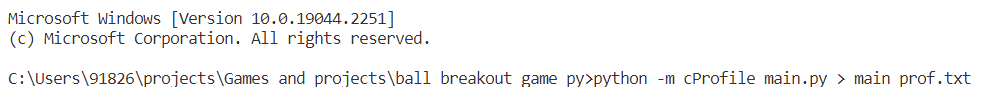
\includegraphics[scale=0.75]{python_main_prof_00}}\end{center}
\begin{center}{\centering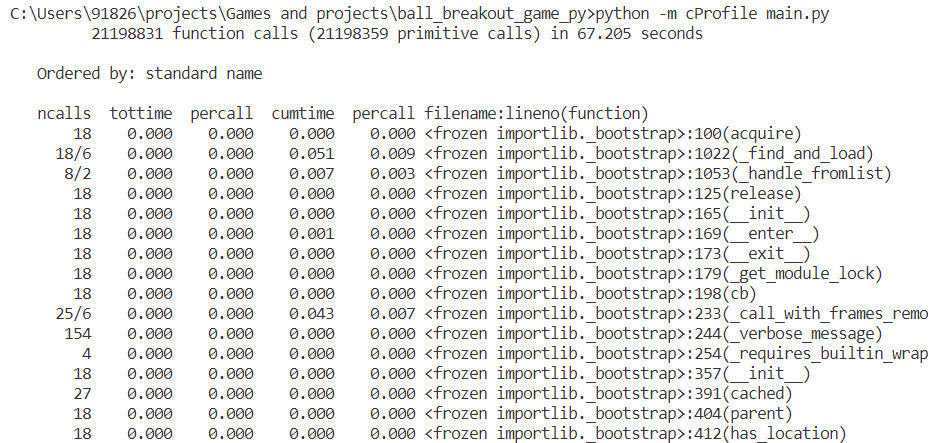
\includegraphics[scale=0.70]{python_main_prof_01}}\end{center}
\begin{center}{\centering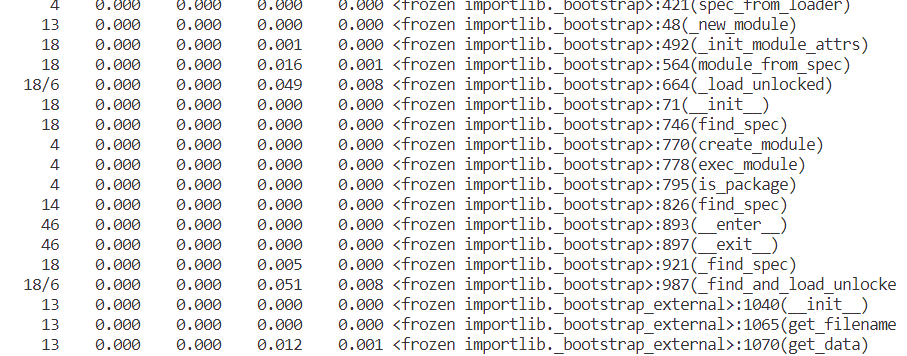
\includegraphics[scale=0.70]{python_main_prof_02}}\end{center}
ball.py
\begin{center}{\centering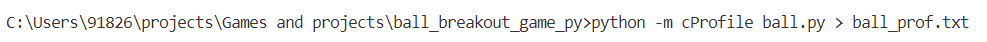
\includegraphics[scale=0.75]{python_ball_prof_00}}\end{center}
\begin{center}{\centering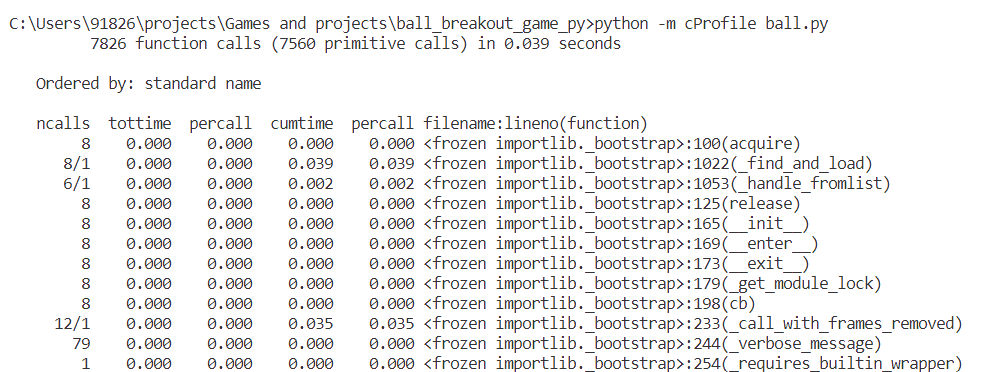
\includegraphics[scale=0.70]{python_ball_prof_01}}\end{center}
\begin{center}{\centering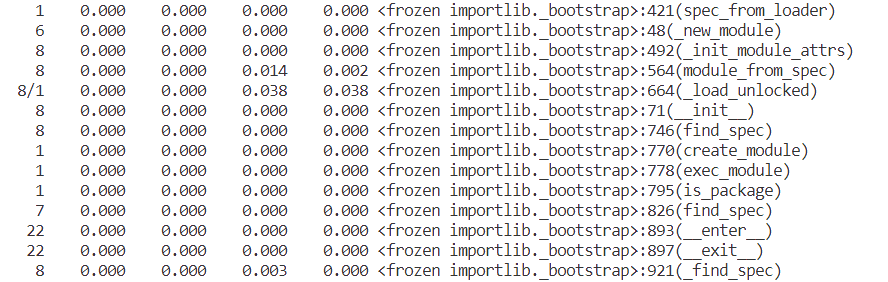
\includegraphics[scale=0.70]{python_ball_prof_02}}\end{center}
bricks.py
\begin{center}{\centering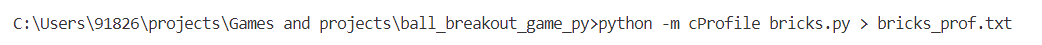
\includegraphics[scale=0.75]{python_bricks_prof_00}}\end{center}
\begin{center}{\centering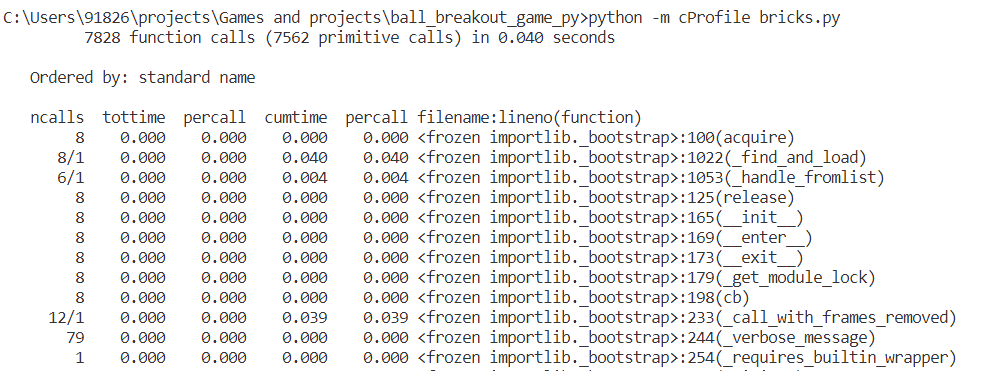
\includegraphics[scale=0.70]{python_bricks_prof_01}}\end{center}
\begin{center}{\centering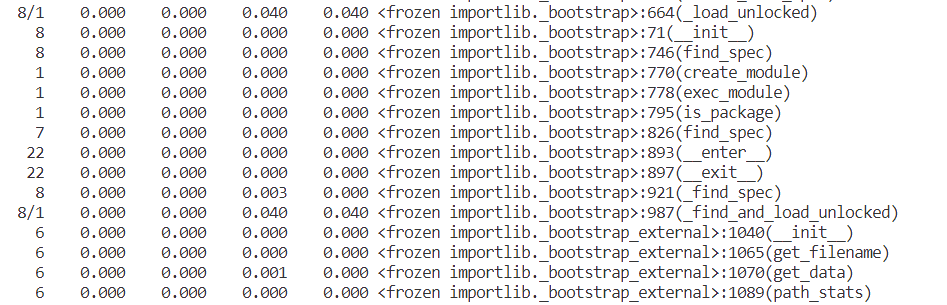
\includegraphics[scale=0.70]{python_bricks_prof_02}}\end{center}
pdle.py
\begin{center}{\centering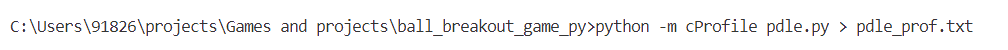
\includegraphics[scale=0.75]{python_pdle_prof_00}}\end{center}
\begin{center}{\centering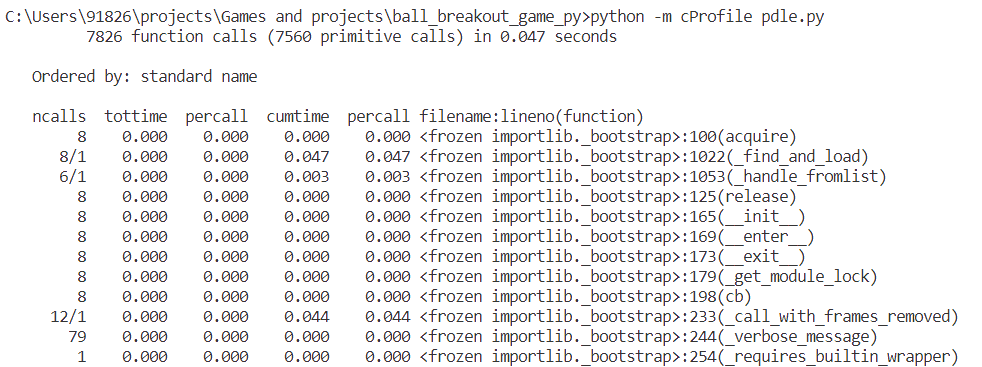
\includegraphics[scale=0.70]{python_pdle_prof_01}}\end{center}
\begin{center}{\centering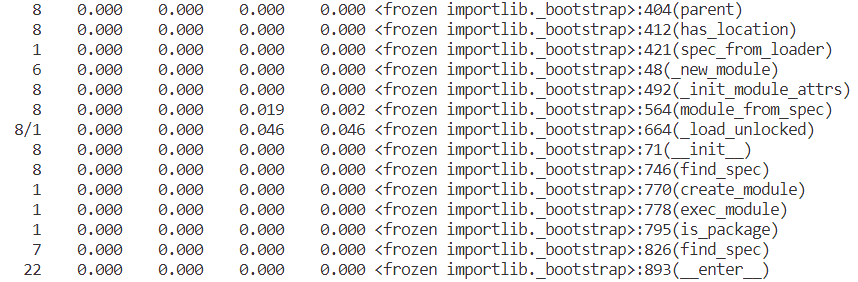
\includegraphics[scale=0.70]{python_pdle_prof_02}}\end{center}
scrbrd.py
\begin{center}{\centering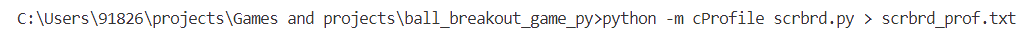
\includegraphics[scale=0.75]{python_scrbrd_prof_00}}\end{center}
\begin{center}{\centering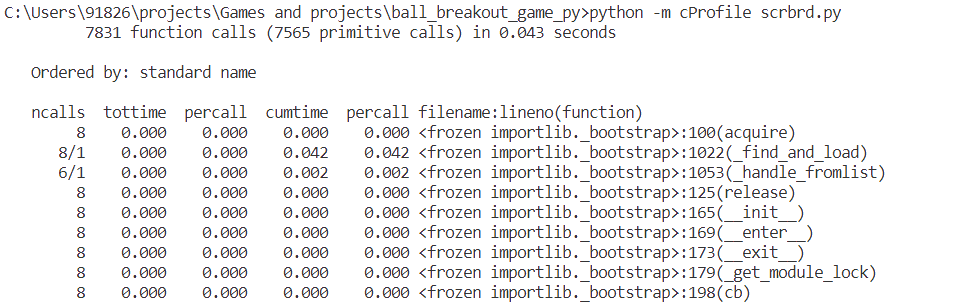
\includegraphics[scale=0.70]{python_scrbrd_prof_01}}\end{center}
\begin{center}{\centering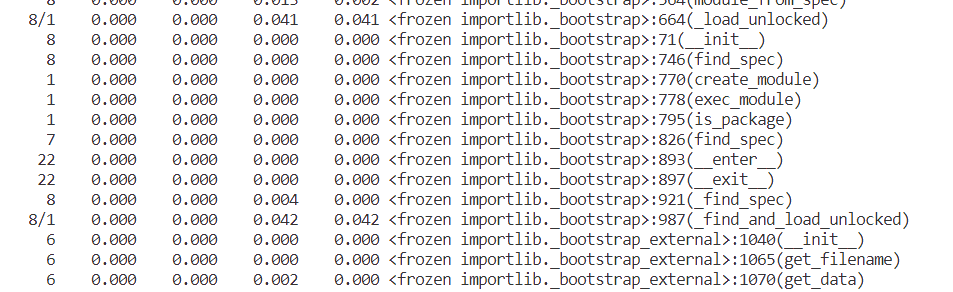
\includegraphics[scale=0.70]{python_scrbrd_prof_02}}\end{center}
ui.py
\begin{center}{\centering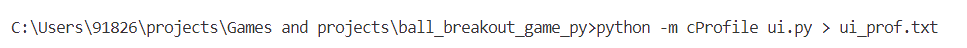
\includegraphics[scale=0.75]{python_ui_prof_00}}\end{center}
\begin{center}{\centering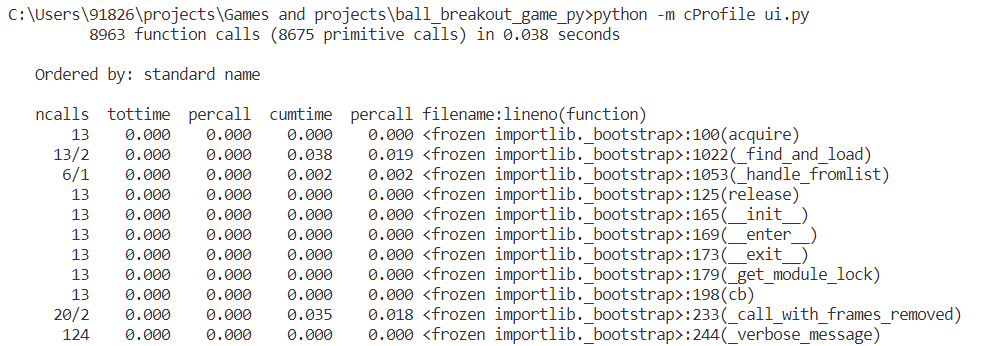
\includegraphics[scale=0.70]{python_ui_prof_01}}\end{center}
\begin{center}{\centering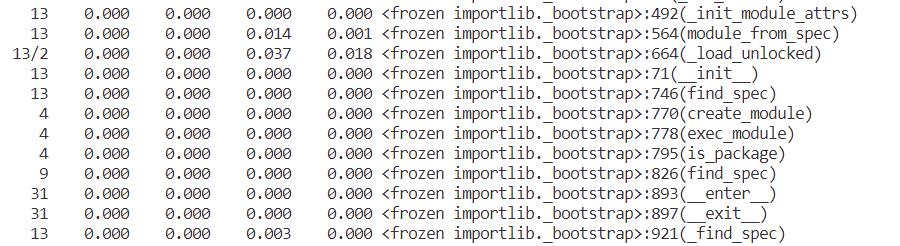
\includegraphics[scale=0.70]{python_ui_prof_02}}\end{center}

\textbf{\bf Debug (Python) : \\}
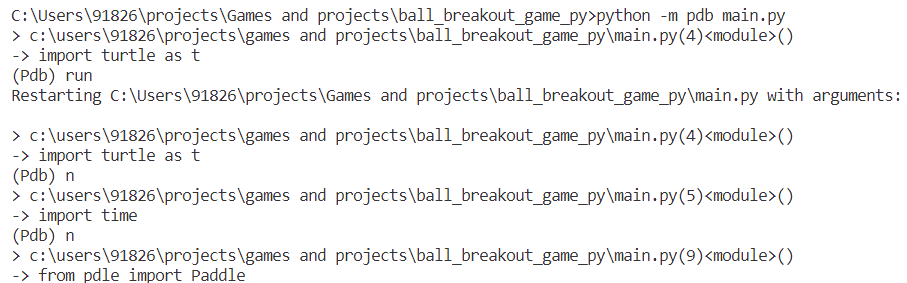
\includegraphics[scale=0.70]{main_pdb_01}\\
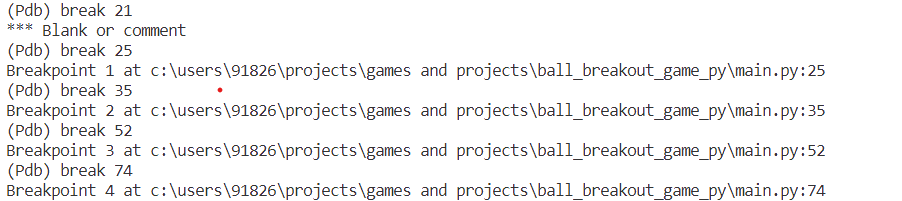
\includegraphics[scale=0.70]{main_pdb_02}\\
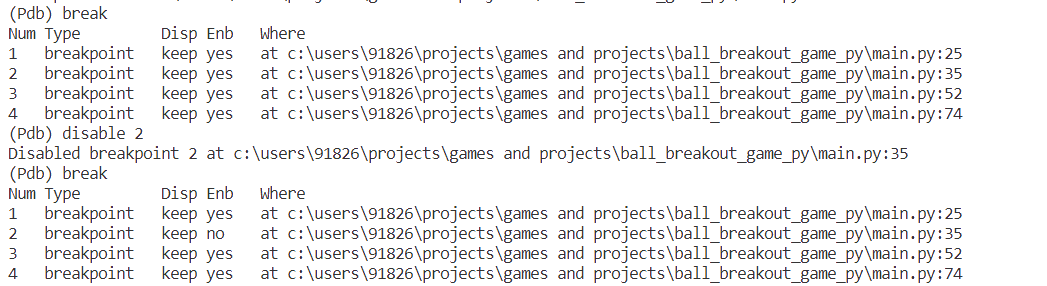
\includegraphics[scale=0.70]{main_pdb_03}\\
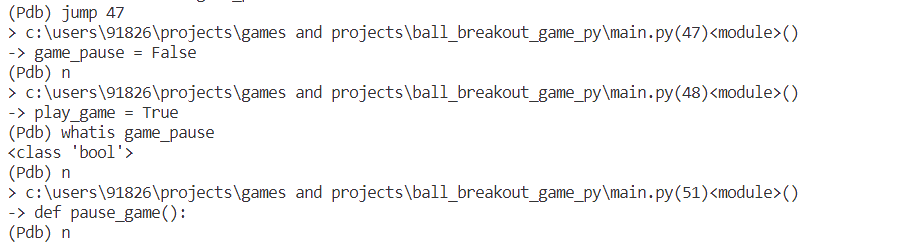
\includegraphics[scale=0.70]{main_pdb_04}\\
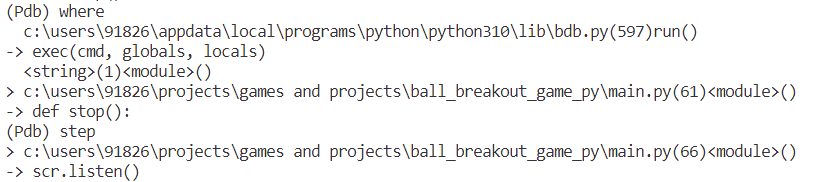
\includegraphics[scale=0.70]{main_pdb_05}\\
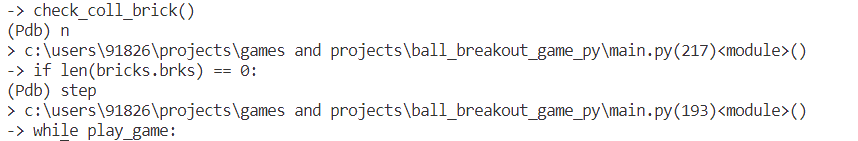
\includegraphics[scale=0.70]{main_pdb_06}\\
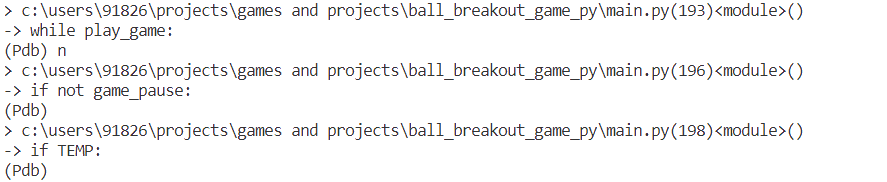
\includegraphics[scale=0.70]{main_pdb_07}\\
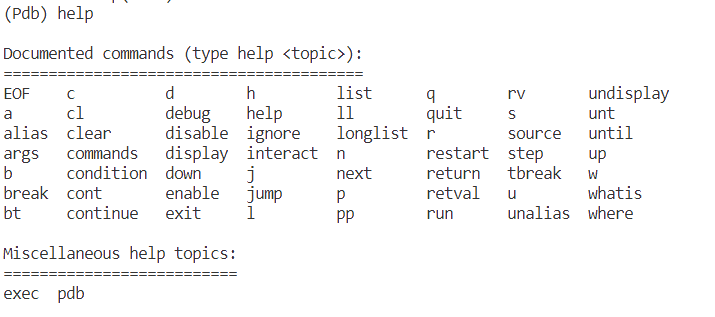
\includegraphics[scale=0.70]{main_pdb_08}\\

\textbf{\bf Code (Python) : \\}

\textbf{\bf main.py}
\lstinputlisting[language = Python]{./main.py}
\textbf{\bf bricks.py}
\lstinputlisting[language = Python]{./bricks.py}
\textbf{\bf pdle.py}
\lstinputlisting[language = Python]{./pdle.py}
\textbf{\bf ball.py}
\lstinputlisting[language = Python]{./ball.py}
\textbf{\bf scrbrd.py}
\lstinputlisting[language = Python]{./scrbrd.py}
\textbf{\bf ui.py}
\lstinputlisting[language = Python]{./ui.py}

\textbf{\bf Ouput (Python) : \\}
\begin{center}{\centering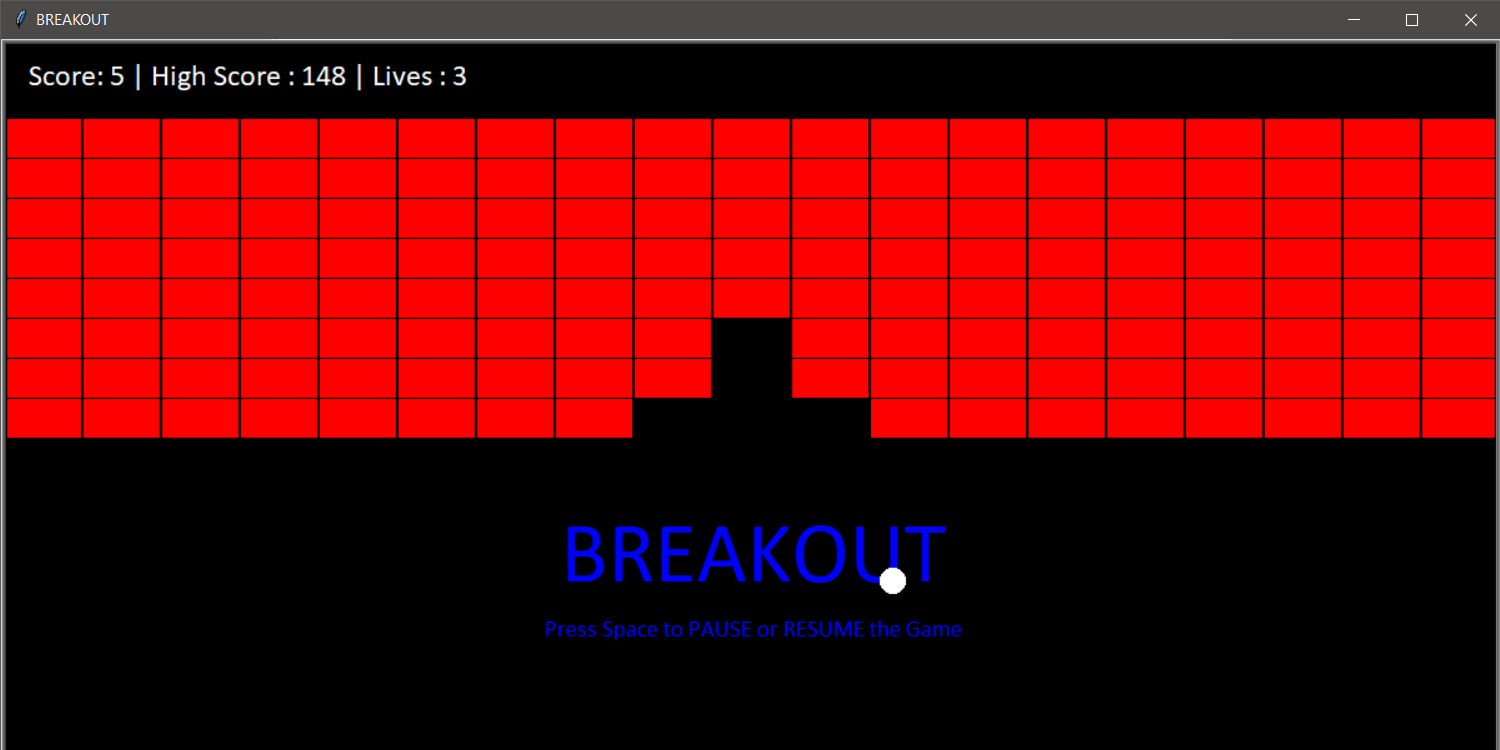
\includegraphics[scale=0.20]{py_out_01}}\end{center}
\begin{center}{\centering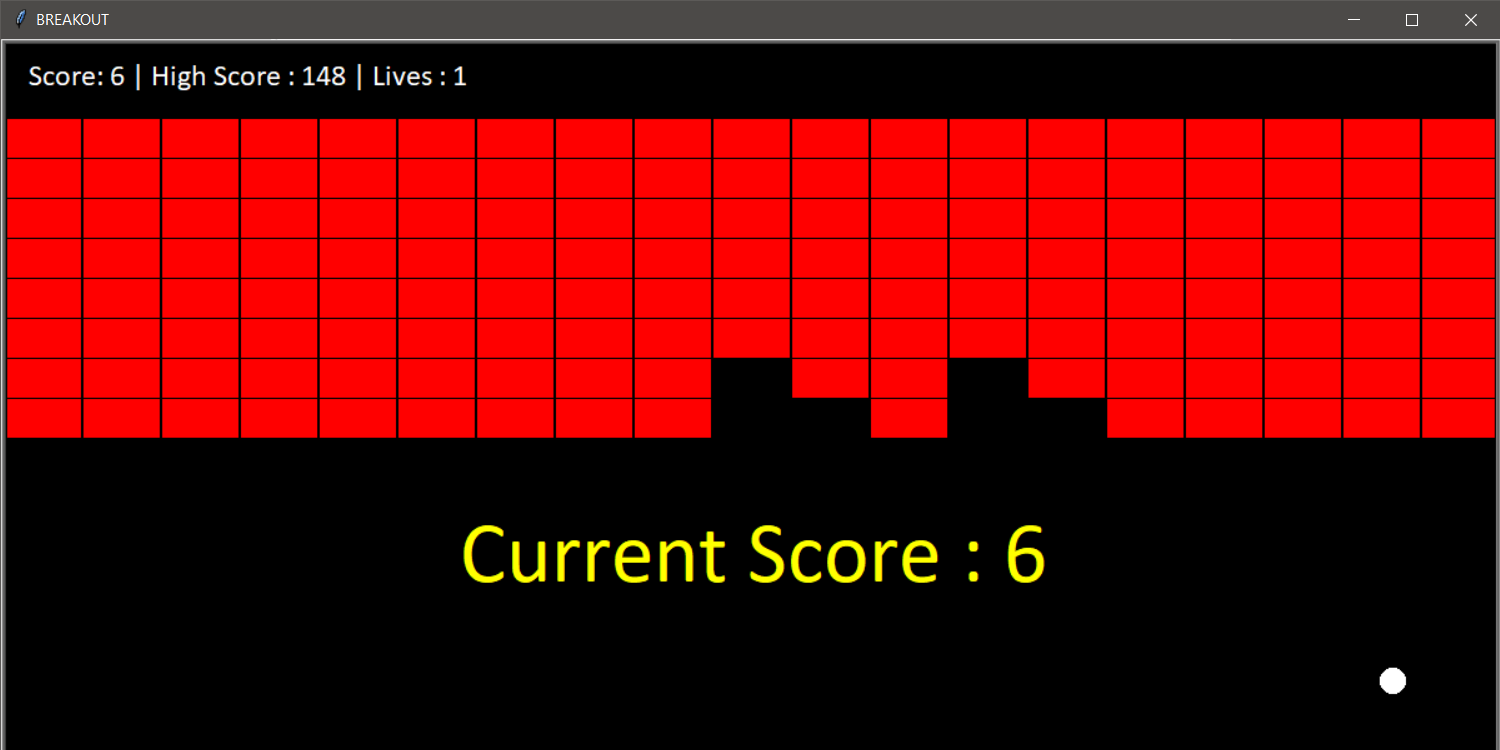
\includegraphics[scale=0.20]{py_out_02}}\end{center}
\begin{center}{\centering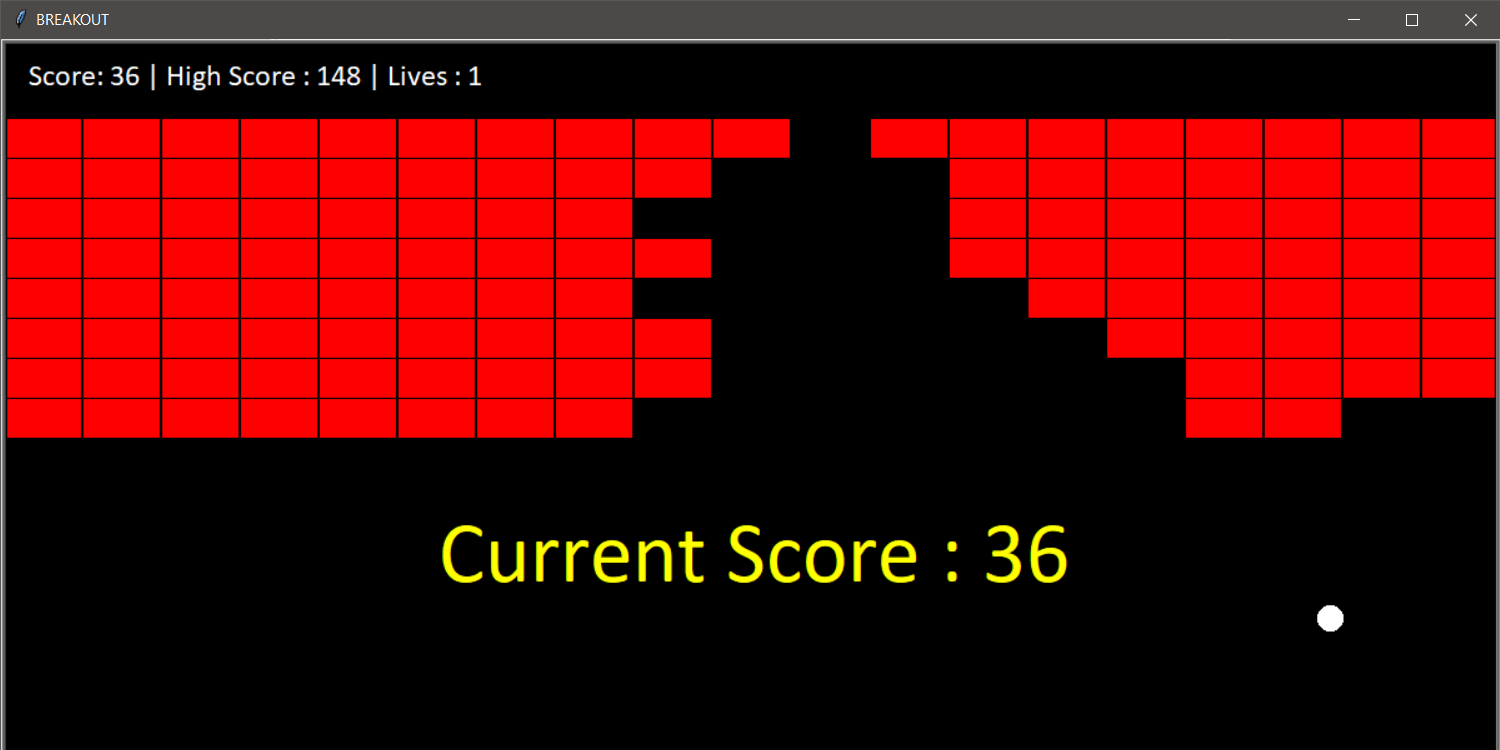
\includegraphics[scale=0.20]{py_out_03}}\end{center}
\begin{center}{\centering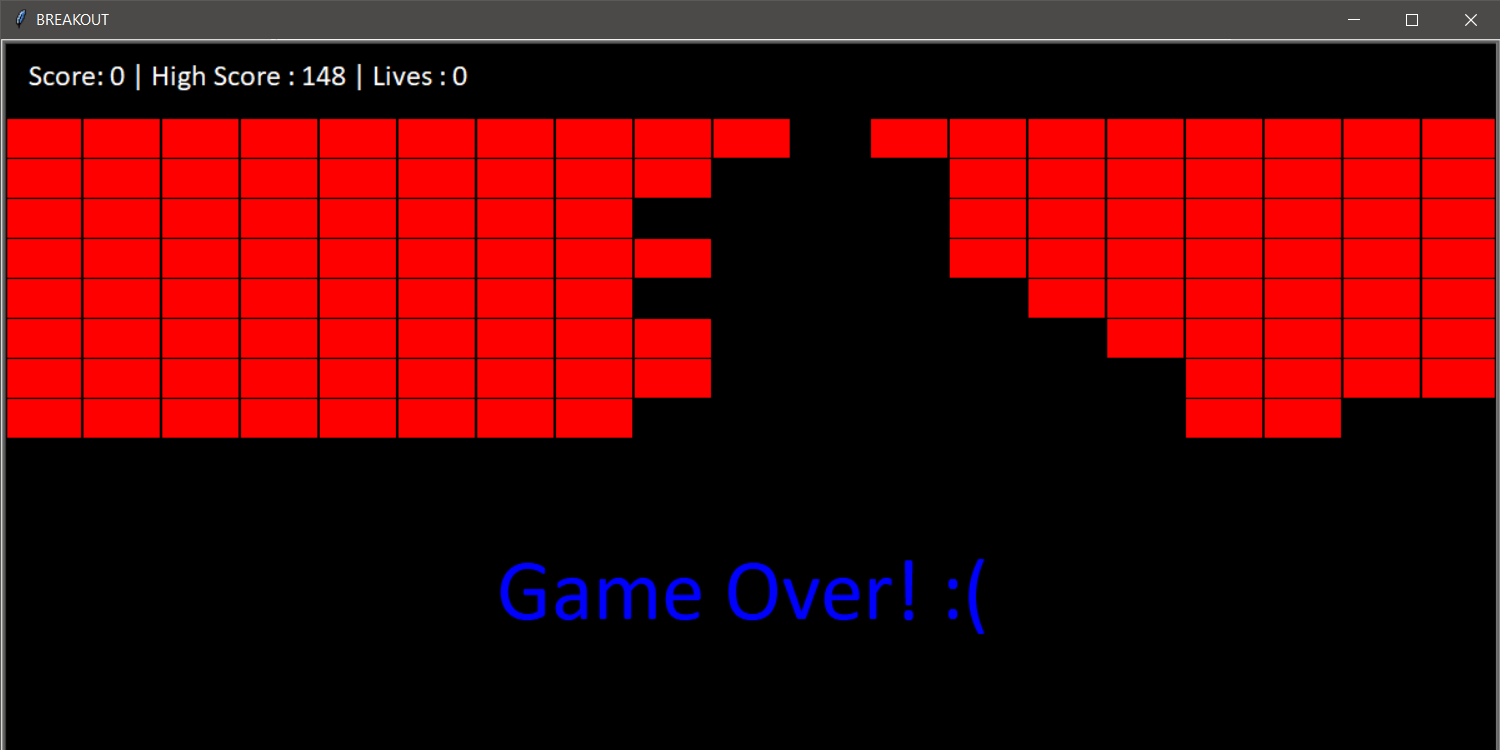
\includegraphics[scale=0.20]{py_out_04}}\end{center}

\pagebreak
\begin{center}{\centering \large{\textbf{\bf SIMPLE CACULATOR\\}}}\end{center}

\textbf{\bf Objective Of Project : \\}
C++ is a cross-platform language that can be used to create high-performance applications.C++ is one of the world's most popular programming languages. C++ can be found in today's operating systems, Graphical User Interfaces, and embedded systems.\par We will create a simple calculator using C++. This calculator will ask the user what operation they want to perform and then act accordingly and give the desired output.\\

\textbf{\bf Statiscal information : \\}
Starting date : 19, November, 2022\\
End Date : 20, November, 2022\\
Total Time Required : 1 day\\
Total Line Of Code (C++): 267 \\
Number Of Funcitons (C++) : 17 \\

\textbf{\bf Function description (C++) : \\}

File : main.cpp\\
1. main : This is the main function used to begin the program.\\

File : interface.h\\
2. interface : This function is used to take the operations from user and check what it is.\\
3. check\_op : This function checks the operation entered by user and then does the appropriate operation.\\

File : operations.h\\
4. add : This function performs addition of 2 given numbers.\\
5. sub : This function performs subtraction of 2 given numbers.\\
6. mul : This funtction multiplies 2 given numbers.\\
7. div : This function divides 2 given numbers.\\
8. percent : This funciton finds num1 percent of num2. Where num1 and num2 are 2 given numbers.\\
9. fact : This function finds factorial of the given non-negative integer.\\
10. nPr : This function finds the permutations of 2 given numbers. Taking the bigger as n and smaller as r in $^{n}P_r$.\\
11. nCr : This function finds the combinations of 2 given numbers. Taking the bigger as n and smaller as r in $^{n}C_r$.\\
12. sqr : This function finds the square the given number. \\
13. cube : This function finds the cube of the given number.\\
14. power : This function finds num1 raised to the power num2. Both given by the user as input.\\
15. sine : This function finds sine of the given number considering to the be argument in radian.\\
16. cosine : This function finds cosine of the given number considering to the be argument in radian.\\
17. tangent : This function finds tangent of the given number considering to the be argument in radian.
\pagebreak

\textbf{\bf Profile Report (C++) : \\}
main.cpp\\
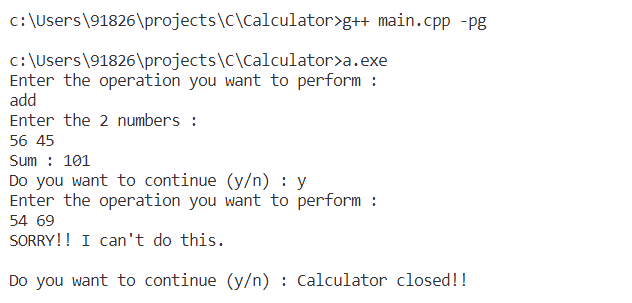
\includegraphics[scale=0.70]{cpp_main_prof_01}\\
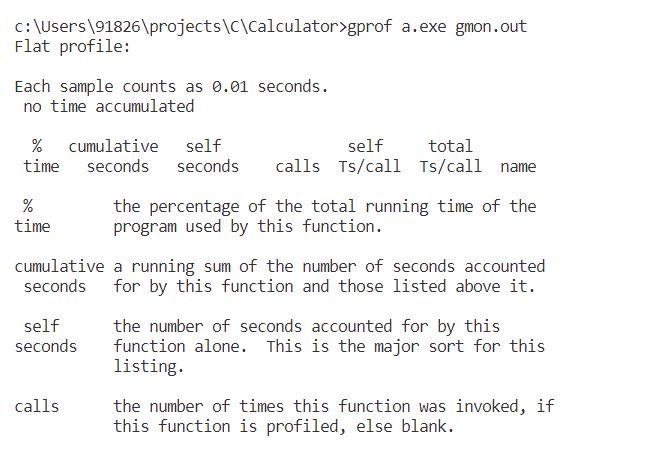
\includegraphics[scale=0.70]{cpp_main_prof_02}\\
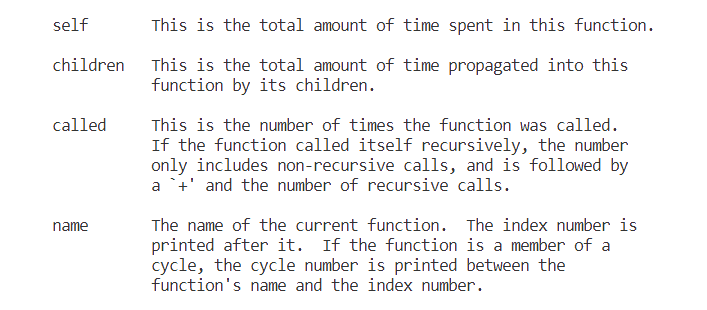
\includegraphics[scale=0.70]{cpp_main_prof_03}\\
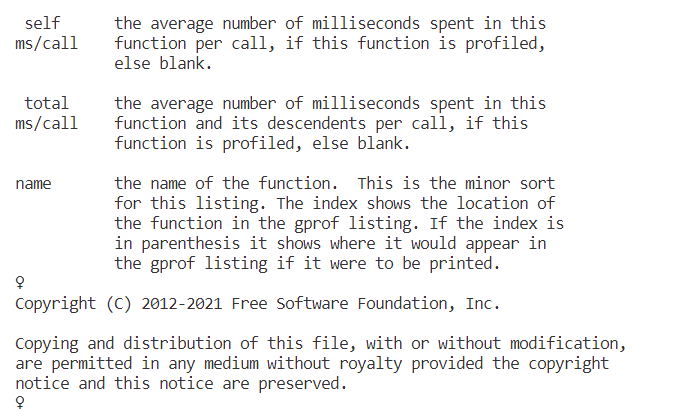
\includegraphics[scale=0.70]{cpp_main_prof_04}\\
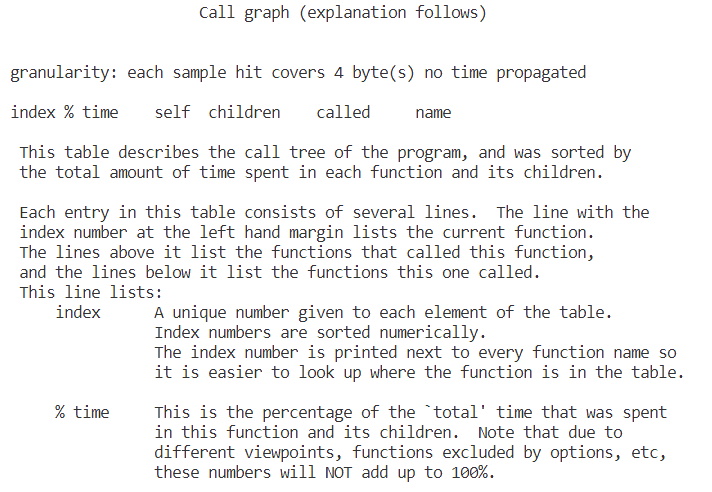
\includegraphics[scale=0.70]{cpp_main_prof_05}\\
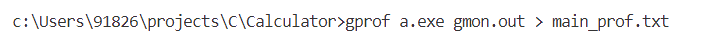
\includegraphics[scale=0.70]{cpp_main_prof_06}\\

\textbf{\bf Debug (C++) : \\}
main.cpp\\
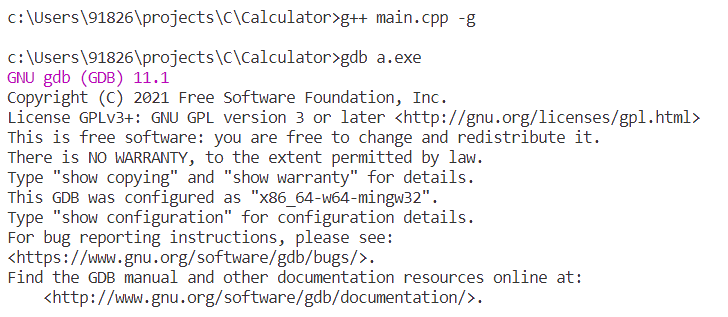
\includegraphics[scale=0.70]{cpp_debug_01}\\
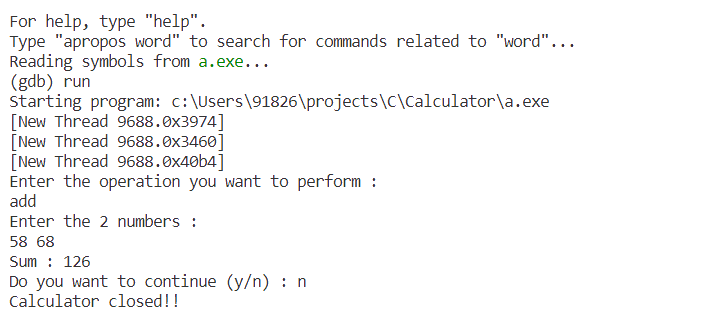
\includegraphics[scale=0.70]{cpp_debug_02}\\
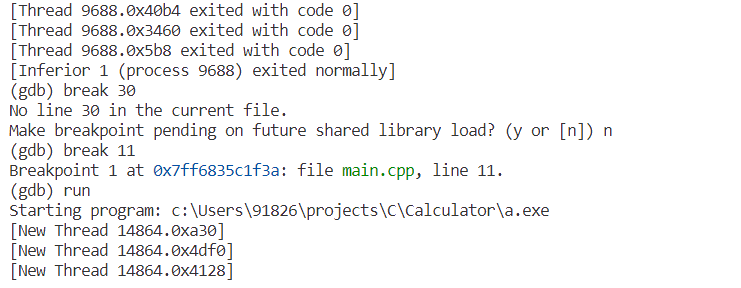
\includegraphics[scale=0.70]{cpp_debug_03}\\
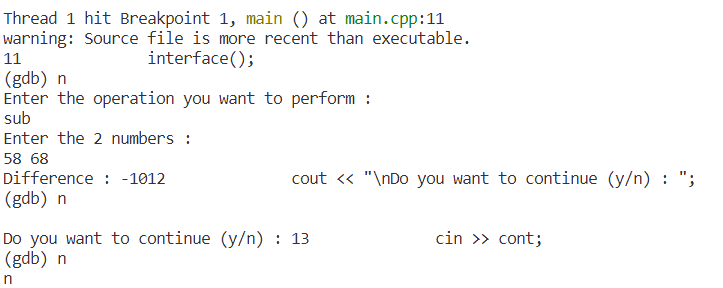
\includegraphics[scale=0.70]{cpp_debug_04}\\
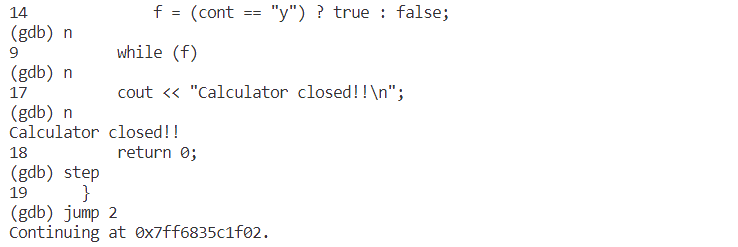
\includegraphics[scale=0.70]{cpp_debug_05}\\
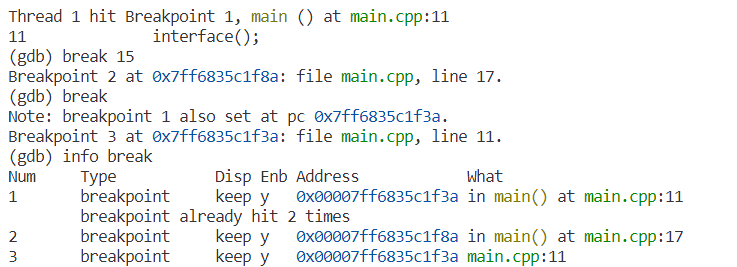
\includegraphics[scale=0.70]{cpp_debug_06}\\
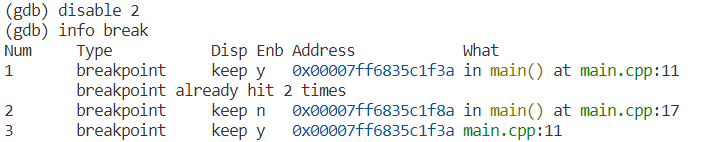
\includegraphics[scale=0.70]{cpp_debug_07}\\
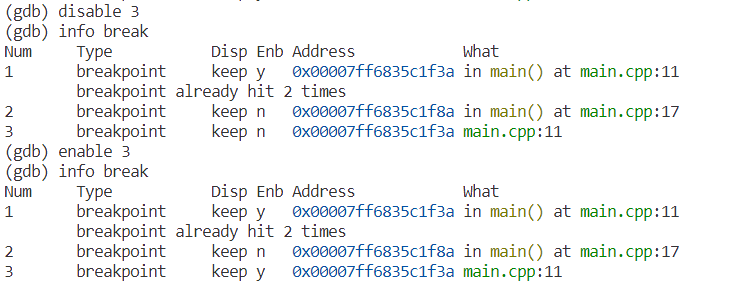
\includegraphics[scale=0.70]{cpp_debug_08}\\
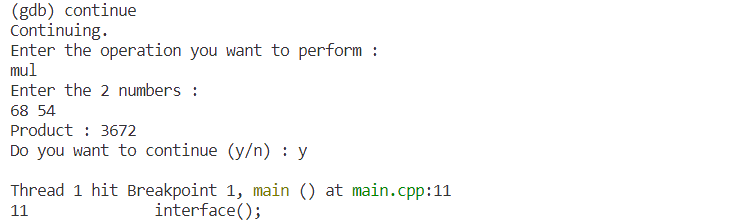
\includegraphics[scale=0.70]{cpp_debug_09}\\
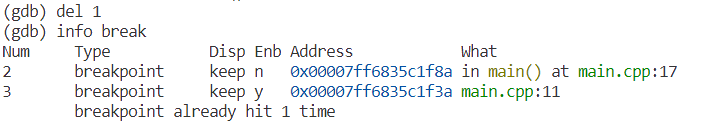
\includegraphics[scale=0.70]{cpp_debug_10}\\
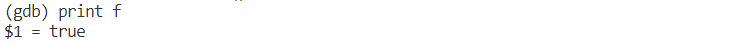
\includegraphics[scale=0.70]{cpp_debug_11}\\
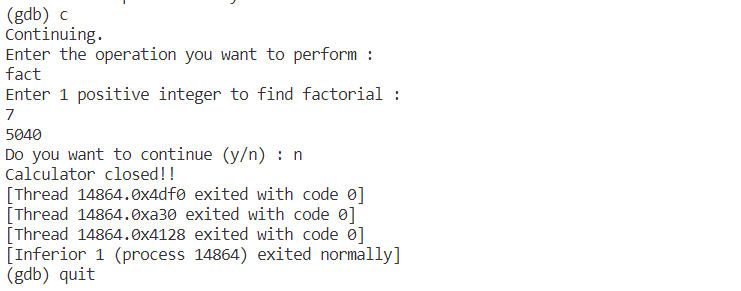
\includegraphics[scale=0.70]{cpp_debug_12}\\

\textbf{\bf Code (C++) : \\}

\textbf{\bf main.cpp}
\lstinputlisting[language = C++]{./main.cpp}
\textbf{\bf interface.h}
\lstinputlisting[language = C++]{./interface.h}
\textbf{\bf operations.h}
\lstinputlisting[language = C++]{./operations.h}
\pagebreak

\textbf{\bf Ouput (C++) : \\}
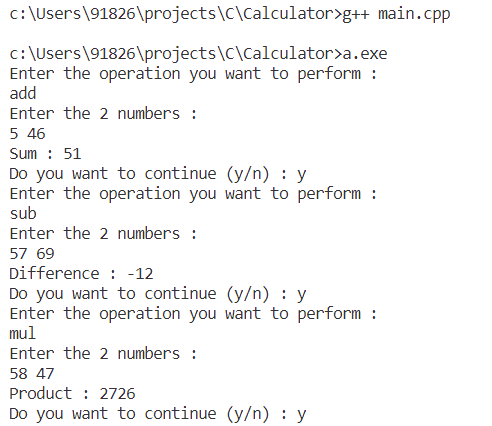
\includegraphics[scale=0.70]{cpp_out_01}\\
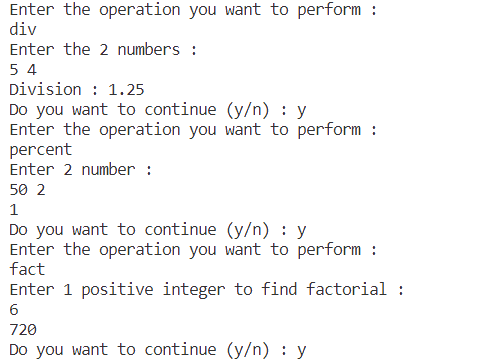
\includegraphics[scale=0.70]{cpp_out_02}\\
\includegraphics[scale=0.70]{cpp_out_03}\\
\includegraphics[scale=0.70]{cpp_out_04}\\
\includegraphics[scale=0.70]{cpp_out_05}\\
\includegraphics[scale=0.70]{cpp_out_06}\\


\end{document}